\section{Introduction}

Although word alignment found its use mainly in phrase-based machine translation (for generating phrase tables), it is still useful for many other tasks and applications: boosting neural MT performance \citep{alkhouli2016alignment}, exploring cross-linguistic phenomena \citep{schrader2006does}, computing quality estimation \citep{specia2013quest}, presenting quality estimation \citep{zouhar2020extending} or simply highlighting matching words and phrases in interactive MT (publicly available MT services).

The aim of this paper is to improve the word alignment quality and demonstrate the capabilities of alignment based on NMT confidence. Closely related to this is the section devoted to aggregating multiple NMT-based alignment models together, which outperforms the individual models.
This is of practical use (better alignment) as well as of theoretical interest (word alignment information encoded in NMT scores). 

We first briefly present the task of word alignment, the metric and the used tools and datasets.
In \Cref{sec:individual} we introduce the soft word alignment models based on MT scores and also several hard word alignment methods (extractors).
The models are evaluated together with other solutions (\fastalign{} and Attention) in \Cref{sec:evaluation}.
We then evaluate the models enhanced with new features and combined together using a simple feed-forward neural network (\Cref{sec:aggregated}).
In both cases, we explore the models' behaviour on Czech-English and German-English datasets.

All of the code is available open-source.\footnotehref{https://github.com/zouharvi/LeverageAlign}{github.com/zouharvi/LeverageAlign}

\subsection{Word Alignment} \label{subsec:word_alignment}

Word alignment (also bitext alignment) is a task of matching two groups of words together that are each other's semantic translation. This is problematic for non-content words which are specific for the given language but generally one is able to construct a mapping as in the example in \Cref{fig:alignment_example}. Word alignment usually follows after sentence alignment.
Even though it is called word alignment, it usually operates on all tokens, including punctuation marks.
%\footnote{Drawn using \href{https://vilda.net/s/slowalign/}{vilda.net/s/slowalign}. More complex word alignment illustrations are available with \href{https://github.com/M4t1ss/SoftAlignments}{github.com/M4t1ss/SoftAlignments}}

\begin{figure*}[ht!]
    \vspace{0.01cm}
    \center
    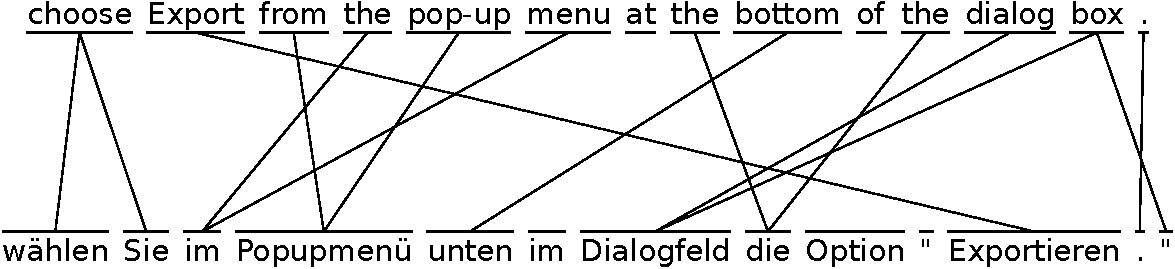
\includegraphics[width=0.87\textwidth]{alignment_example.pdf}
    \caption{
        Illustration of English (top) to German (bottom) word alignment. The token >>choose<< is aligned to two tokens >>wählen<< and >>Sie<< while the token >>Option<< is left unaligned. The article >>die<< is mistakenly aligned to two unrelated articles >>the<<.
        \label{fig:alignment_example}
    }
    \vspace{0.2cm}
\end{figure*}

Word alignment output can be formalized as a set containing tuples of source-target words. For an aligner output $A$, a sure alignment $S$ and a possible alignment $P$ ($S\subseteq P$),\footnote{Sure alignments can be treated as gold alignments with very high confidence, while pairs marked with possible alignments are still sensible to connect, but with the decision being much less clear. The AER is designed not to penalize models by including more possible alignments in the gold annotations.} precision can be computed as $ \frac{|A \cap P|}{|A|}$ and recall as $\frac{|A \cap S|}{|S|}$. The most common metric, Alignment Error Rate (AER), is defined as $1-\frac{|A\cap S| + |A \cap P|}{|S|+|A|}$ (lower is better). Even though the test set is annotated with two types of alignments, the aligner is expected to produce only one type. These evaluation measures are described by \citet{mihalcea2003evaluation} and \citet{och2003systematic}.

Traditionally word alignment models can be split into soft and hard alignment parts. In soft alignment, the model produces a score for every source-target pair. When producing hard alignment (extractors), the model makes decisions as to which alignments to include in the output. For source sentence $S$ and target sentence $T$, the output of soft alignment is a $\mathbb{R}^{|S|\times|T|}$ matrix while hard alignment is a set $A \subseteq S\times T$.


\paragraph{Symmetrization.}

Assuming that we have access to bi-directional word alignment (in the context of this paper to two MT systems of the opposite directions) we can compute both the alignment from source to target ($X$) and target to source ($X'$).
Having access to both $X$ and $X'$ makes it possible to create a new alignment $Y$ with either higher precision through intersection or higher recall through union \citep{koehn2009statistical}.
\begin{gather*}
    X^T := \{(b, a): (a, b) \in X\} \\
    Y_{prec} = X \cap X'^T \qquad Y_{rec} = X \cup X'^T
\end{gather*}

We can make use of the fact that the models output soft alignment scores and create new alignment scores in the following way using a simple linear regression model. This allows us to fine-tune the relevance of each of the directions as well as their interaction. However, it does not have the same effects as the union or the intersection because it affects the soft alignment and not hard alignment in contrast to the previous case.
\begin{gather*}
    p^{sym}(s,t) = \beta_0 \cdot p(s, t) + \beta_1 \cdot p^r(t, s) + \beta_2 \cdot p(s, t) \cdot p^r(t, s)
\end{gather*}

More complex symmetrization techniques have been proposed and implemented by \citet{och2000improved, junczys2011symgiza++}.

\subsection{Relevant Work}

\citet{och2003systematic} introduce the word alignment task and systematically compare the IBM word alignment models.
The work of \citet{li2019word} is closely related to this article as it examines the issue of word alignment from NMT and proposes two ways of extracting it: prediction difference and explicit model. They also show that without guided alignment in training, NMT systems perform worse than \fastalign{} baseline.
Using attention for word alignment is thoroughly discussed by \citet{bahdanau2014neural} and \citet{zenkel2019adding}.
Word alignment based on static and contextualized word embeddings is explored by the recent work of \citet{sabet2020simalign}.
Word alignment based on cross-lingual (more than 2 languages) methods is presented by \citet{wu2021slua}.
The work of \citet{chen2020accurate} focuses on inducing word alignments from glass-box NMT as a replacement for using Transformer attention layers directly.
\citet{chen2020mask} document Mask Align, an unsupervised neural word aligner based on a single masked token prediction.

\citet{chen2016guided} propose guided attention, a mechanism that uses word alignment to bias the attention during training. This improves the MT performance on especially rare and unknown tokens. The usage of word alignment in this work is, however, opposite to the goals of this paper. While for \citet{chen2016guided} the word alignment improved their MT system, here the MT system improves the word alignment.


\subsection{Tools}

The experiments in this paper require an MT system capable of providing output probabilities (decoder scores) and optionally also attention-based word alignment. For comparison, we also use an IBM-model-based word aligner. This tool is also used as an additional feature to the final aggregation model.

\paragraph{MarianNMT}\hspace{-0.25cm} \citep{junczys2018marian, junczys2018marian2} is a popular (both in academia and in deployment scenarios), actively developed and maintained system for fast machine translation. It already contains options for producing word alignment, output probabilities for words and sentences and also attention scores.

\paragraph{\fastalign}\hspace{-0.25cm} \citep{dyer2013simple} is an unsupervised word aligner based on IBM Alignment Model 2. It does not provide state of the art pre-neural performance but is easy to build with modern toolchains and has low resource requirements (both memory- and computational-wise).

\subsection{Data}

For training purposes, we make use mostly of the parallel corpora of Czech--English word alignments by \citet{marecek_csen_algn_corpus}, based on manually annotated data. We also include a large Czech-English corpus by \citet{czeng2} and a large German--English corpus by \citet{rozis_tilde}, which are not word aligned. From this corpus, 1M sentences were sampled randomly. A small manually aligned German--English corpus by \citet{bicini_ende_algn_corpus} is included for testing. An overview of the corpus sizes is displayed in \Cref{tab:corpus_used}.

\begin{table*}[h!]
    \center
    \begin{tabular}{lccrrr}
        \toprule
        CS/DE-English & Type &\hspace{-0.1cm}Domain &\hspace{-0.1cm}CS/DE Tok. & EN Tok. & Sent. \\
        \cmidrule{1-6}
        Czech Small & aligned & news, legal & 53k & 60k & 2.5k \\
        Czech Big & unaligned & multi & 2618M & 3013M & 188M \\
    German Small\hspace{-0.2cm} & aligned & legal & 1k & 1k & 0.1k \\
        German Big & unaligned &tech, news, legal & 23M & 25M & 1M \\
        \bottomrule
    \end{tabular}
    \caption{Used word aligned corpora with their sizes, domains and origin. \label{tab:corpus_used}}
\end{table*}

\subsection{MT Models}

We make use of the MT models made available\footnotehref{https://github.com/browsermt/students}{github.com/browsermt/students} by \citet{model_csen} and \citet{model_deen}. For both Czech-English and English-German, CPU-optimized student models are used. They are transformer-based \citep{vaswani2017transformer} and were created by using knowledge distillation. With WMT19 and WMT20 SacreBLEU \citep{sacrebleu}, the models achieve the following BLEU scores: Czech-English (27.7), English-Czech (36.3) and English--German (42.7).\footnote{%
BLEU+case.mixed+lang.cs-en+numrefs.1 +smooth.exp+test.wmt20+tok.13a+version.1.4.13\\
\hspace*{0.49cm}BLEU+case.mixed+lang.en-cs+numrefs.1 +smooth.exp+test.wmt20+tok.13a+version.1.4.13\\
\hspace*{0.49cm}BLEU+case.mixed+lang.en-de+numrefs.1+smooth.exp+test.wmt19+tok.13a+version.1.4.8} Since the English--German MT is only available in one direction, word alignment is reported in this direction as well. Exceptions, such as word alignment using an MT for the opposite direction, are explicitly mentioned.